%% AMS-LaTeX Created with the Wolfram Language : www.wolfram.com

\documentclass{article}
\usepackage{amsmath, amssymb, graphics, setspace}

\newcommand{\mathsym}[1]{{}}
\newcommand{\unicode}[1]{{}}

\newcounter{mathematicapage}
\begin{document}

\begin{doublespace}
\noindent\(\pmb{\text{ket0}=\text{SparseArray}[\{\{1,1\}\to 1,\{2,1\}\to 0\}];\text{ket1}=\text{SparseArray}[\{\{2,1\}\to 1\}];}\)
\end{doublespace}

\begin{doublespace}
\noindent\(\pmb{g=\text{Graph}[\{1\text{-$>$}2,1\text{-$>$}3,1\text{-$>$}4,2\text{-$>$}1,2\text{-$>$}4,3\text{-$>$}4,4\text{-$>$}3\}]; \text{(*}\text{Grafo}\text{*)}}\\
\pmb{\text{(*}g=\text{Graph}[\{1\text{-$>$}2,1\text{-$>$}3,2\text{-$>$}4\}];\text{*)} \text{(*Grafo {\' a}rbol*)}}\\
\pmb{\text{(*}g=\text{Graph}[\{1\text{-$>$}2,1\text{-$>$}3,1\text{-$>$}4,2\text{-$>$}1,3\text{-$>$}1,4\text{-$>$}1\}];\text{*)} \text{(*Grafo estrella*)}}\\
\pmb{\text{(*}g=\text{Graph}[\{1\text{-$>$}2,2\text{-$>$}3,3\text{-$>$}1, 1\text{-$>$}3,3\text{-$>$}2,2\text{-$>$}1, 1\text{-$>$}4,2\text{-$>$}4,3\text{-$>$}4\}];\text{*)}
}\\
\pmb{\text{(*Grafo corona*)}}\)
\end{doublespace}

\begin{doublespace}
\noindent\(\pmb{\text{Em}=\text{AdjacencyMatrix}[g]; }\\
\pmb{\text{For}[j=1,j\text{$<$=}4,j\text{++},}\\
\pmb{\quad \text{OutDeg}=\text{Sum}[\text{Em}[[j,i]],\{i,1,4\}];}\\
\pmb{\quad \text{If}[\text{OutDeg}\text{!=}0, \text{Em}[[j]]=\text{Em}[[j]]/\text{OutDeg}, \text{Em}[[j]]=\{1/4,1/4,1/4,1/4\};]]}\\
\pmb{\text{Em}=\text{Transpose}[\text{Em}]; }\\
\pmb{\text{(*Matriz de adyacencia del grafo*)}}\)
\end{doublespace}

\begin{doublespace}
\noindent\(\pmb{G=\alpha  \text{Em} + \frac{(1-\alpha )}{\text{Dimensions}[\text{Em}][[1]]} \text{Table}[1,\{\text{Dimensions}[\text{Em}][[1]]\},\{\text{Dimensions}[\text{Em}][[1]]\}];
\text{(*Matriz de Google*)}}\)
\end{doublespace}

\begin{doublespace}
\noindent\(\pmb{\text{Ivl1}=\{1\}; \text{(*PageRank inicial de cada nodo*)}}\\
\pmb{\text{Ivl2}=\{0\};}\\
\pmb{\text{Ivl3}=\{0\};}\\
\pmb{\text{Ivl4}=\{0\};}\\
\pmb{\text{Iv}=\{\{1\},\{0\},\{0\},\{0\}\}; \text{(*Vector de PageRank inicial*)}}\\
\pmb{\text{For}[i=1,i\leq 30,i\text{++},}\\
\pmb{\text{Iv}=(G\text{/.}\{\alpha \to 0.85\}).\text{Iv}; \text{(*Iterar con la matriz de Google*)}}\\
\pmb{\text{(*}\text{Iv}=\text{Iv}/\text{Norm}[\text{Iv}];\text{*)}}\\
\pmb{\text{AppendTo}[\text{Ivl1},\text{Iv}[[1,1]]];}\\
\pmb{\text{AppendTo}[\text{Ivl2},\text{Iv}[[2,1]]];}\\
\pmb{\text{AppendTo}[\text{Ivl3},\text{Iv}[[3,1]]];}\\
\pmb{\text{AppendTo}[\text{Ivl4},\text{Iv}[[4,1]]];]}\)
\end{doublespace}

\begin{doublespace}
\noindent\(\pmb{\text{ListLinePlot}[\text{Ivl1},\text{PlotRange}\to \{0,1\},\text{DataRange}\to \{0,30\}] \text{(*Graficar evoluci{\' o}n del PageRank
de cada nodo*)}}\\
\pmb{\text{ListLinePlot}[\text{Ivl2},\text{PlotRange}\to \{0,1\},\text{DataRange}\to \{0,30\}]}\\
\pmb{\text{ListLinePlot}[\text{Ivl3},\text{PlotRange}\to \{0,1\},\text{DataRange}\to \{0,30\}]}\\
\pmb{\text{ListLinePlot}[\text{Ivl4},\text{PlotRange}\to \{0,1\},\text{DataRange}\to \{0,30\}]}\)
\end{doublespace}

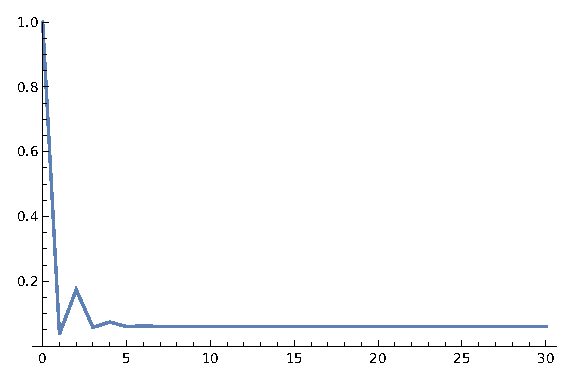
\includegraphics{PageRank_gr1.eps}

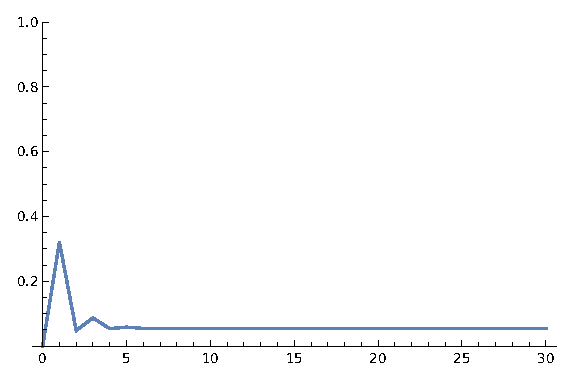
\includegraphics{PageRank_gr2.eps}

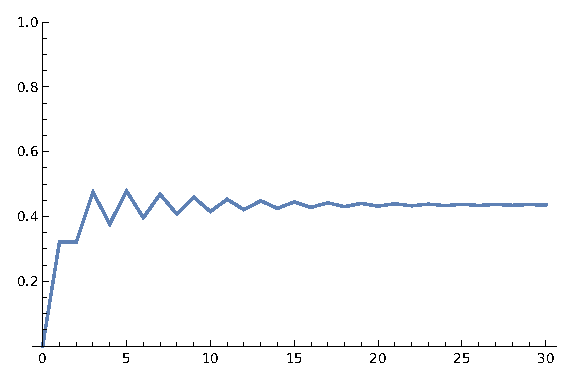
\includegraphics{PageRank_gr3.eps}

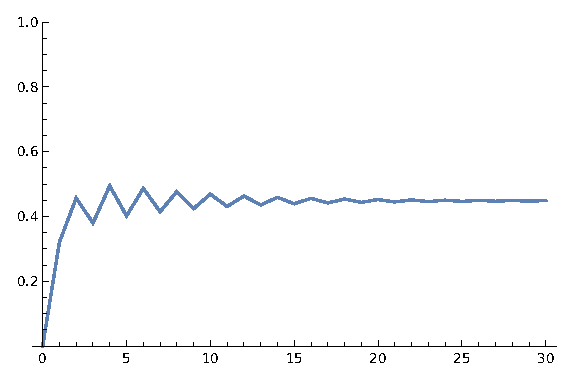
\includegraphics{PageRank_gr4.eps}

\begin{doublespace}
\noindent\(\pmb{\text{PageRankCentrality}[g,0.85] \text{(*Comparar con el PageRank dado por la funci{\' o}n de Mathematica*)}}\)
\end{doublespace}

\begin{doublespace}
\noindent\(\{0.0607532,0.0547134,0.435982,0.448551\}\)
\end{doublespace}

\begin{doublespace}
\noindent\(\pmb{\text{ket}[\text{k$\_$},\text{n$\_$}]\text{:=}\text{Table}[\{i==k\},\{i,0,n-1\}]\text{/.}\{\text{True}\to 1,\text{False}\to 0\};
\text{(*}\text{Generador} \text{de} \text{kets}: k \to  \text{estado}, n \to  \text{dimensi{\' o}n}\text{*)}}\)
\end{doublespace}

\begin{doublespace}
\noindent\(\pmb{\text{$\phi $x}_{\text{j$\_$}}\text{:=}\text{KroneckerProduct}\left[\text{ket}[j-1,4],\text{Sum}\left[\sqrt{G[[k,j]]} \text{ket}[k-1,4],\{k,1,4\}\right]\right];
\text{(*}\text{Estados} A \to  B\text{*)}}\\
\pmb{\text{$\psi $y}_{\text{j$\_$}}\text{:=}\text{KroneckerProduct}\left[\text{Sum}\left[\sqrt{G[[k,j]]} \text{ket}[k-1,4],\{k,1,4\}\right],\text{ket}[j-1,4]\right];
\text{(*}\text{Estados} B \to  A\text{*)}}\\
\pmb{\text{$\phi $x0}=\left.\text{Sum}\left[\text{$\phi $x}_j,\{j,1,4\}\right]\right/2; \text{(*}\text{Superposici{\' o}n} \text{de} \text{los} \text{estados}
A \to  B\text{*)}}\\
\pmb{\text{$\psi $y0}=\left.\text{Sum}\left[\text{$\psi $y}_j,\{j,1,4\}\right]\right/2; \text{(*}\text{Superposici{\' o}n} \text{de} \text{los} \text{estados}
B \to  A\text{*)}}\\
\pmb{\text{$\Pi $x}=\text{Sum}\left[\text{$\phi $x}_j.\text{$\phi $x}_j\dagger,\{j,1,4\}\right]; \text{(*}\text{Proyector} A \to  B\text{*)}}\\
\pmb{\text{$\Pi $y}=\text{Sum}\left[\text{$\psi $y}_j.\text{$\psi $y}_j\dagger,\{j,1,4\}\right]; \text{(*}\text{Proyector} B \to  A\text{*)}}\\
\pmb{S=\text{Sum}[\text{KroneckerProduct}[\text{ket}[j,4],\text{ket}[k,4]].\text{KroneckerProduct}[\text{ket}[k,4],\text{ket}[j,4]]\dagger,\{j,0,3\},\{k,0,3\}];
\text{(*Operador SWAP*)}}\\
\pmb{\text{Ux}=S.(2\text{$\Pi $x}-\text{IdentityMatrix}[16]); \text{(*}\text{Operador} \text{de} \text{difusi{\' o}n} 1/2\text{*)}}\\
\pmb{\text{Ax}=\text{Sum}\left[\text{$\phi $x}_j.\text{ket}[j-1,4]\dagger,\{j,1,4\}\right]; \text{(*A $\to $ B*)}}\\
\pmb{\text{By}=\text{Sum}\left[\text{$\psi $y}_j.\text{ket}[j-1,4]\dagger,\{j,1,4\}\right]; \text{(*B $\to $ A*)}}\\
\pmb{H=\text{HadamardMatrix}[2]; \text{(*}\text{Hadamard}\text{*)}}\\
\pmb{s=\text{KroneckerProduct}[H,H,H,H].\text{KroneckerProduct}[\text{ket}[0,2],\text{ket}[0,2],\text{ket}[0,2],\text{ket}[0,2]]\text{//}N; \text{(*Estado
de superposici{\' o}n uniforme*)}}\\
\pmb{W=(\text{IdentityMatrix}[16]-2 \text{Ax}.\text{Ax}\dagger).(2 s.s\dagger-\text{IdentityMatrix}[16]); \text{(*}\text{Operador} \text{de} \text{difusi{\'
o}n} \text{m{\' a}s} \text{Grover}-\text{like}\text{*)}}\\
\pmb{W=(2 \text{By}.\text{By}\dagger-\text{IdentityMatrix}[16]).(2 \text{Ax}.\text{Ax}\dagger-\text{IdentityMatrix}[16]); \text{(*Operador de difusi{\'
o}n 2*)}}\\
\pmb{W=\text{MatrixPower}[\text{Ux},2]; \text{(*Operador de difusi{\' o}n 1*)}}\\
\pmb{\text{(*}W=\text{MatrixPower}\left[W\text{/.}\alpha \to 0.99,\frac{1}{10}\right];\text{*)}}\)
\end{doublespace}

\begin{doublespace}
\noindent\(\pmb{a=0.85;}\\
\pmb{\text{qIvl1}=}\\
\pmb{\text{Table}[((\text{$\phi $x0}\dagger\text{/.}\{\alpha \to a\}).\text{MatrixPower}[(W\dagger\text{/.}\{\alpha \to a\}),m].\text{KroneckerProduct}[\text{IdentityMatrix}[4],\text{ket}[0,4].\text{ket}[0,4]\dagger].\text{MatrixPower}[(W\text{/.}\{\alpha
\to a\}),m].(\text{$\phi $x0}\text{/.}\{\alpha \to a\}))[[}\\
\pmb{1,1]],\{m,1,30\}];}\\
\pmb{\text{qIvl2}=}\\
\pmb{\text{Table}[((\text{$\phi $x0}\dagger\text{/.}\{\alpha \to a\}).\text{MatrixPower}[(W\dagger\text{/.}\{\alpha \to a\}),m].\text{KroneckerProduct}[\text{IdentityMatrix}[4],\text{ket}[1,4].\text{ket}[1,4]\dagger].\text{MatrixPower}[(W\text{/.}\{\alpha
\to a\}),m].(\text{$\phi $x0}\text{/.}\{\alpha \to a\}))[[}\\
\pmb{1,1]],\{m,1,30\}];}\\
\pmb{\text{qIvl3}=}\\
\pmb{\text{Table}[((\text{$\phi $x0}\dagger\text{/.}\{\alpha \to a\}).\text{MatrixPower}[(W\dagger\text{/.}\{\alpha \to a\}),m].\text{KroneckerProduct}[\text{IdentityMatrix}[4],\text{ket}[2,4].\text{ket}[2,4]\dagger].\text{MatrixPower}[(W\text{/.}\{\alpha
\to a\}),m].(\text{$\phi $x0}\text{/.}\{\alpha \to a\}))[[}\\
\pmb{1,1]],\{m,1,30\}];}\\
\pmb{\text{qIvl4}=}\\
\pmb{\text{Table}[((\text{$\phi $x0}\dagger\text{/.}\{\alpha \to a\}).\text{MatrixPower}[(W\dagger\text{/.}\{\alpha \to a\}),m].\text{KroneckerProduct}[\text{IdentityMatrix}[4],\text{ket}[3,4].\text{ket}[3,4]\dagger].\text{MatrixPower}[(W\text{/.}\{\alpha
\to a\}),m].(\text{$\phi $x0}\text{/.}\{\alpha \to a\}))[[}\\
\pmb{1,1]],\{m,1,30\}];}\)
\end{doublespace}

\begin{doublespace}
\noindent\(\pmb{\text{ListLinePlot}[\text{qIvl1},\text{PlotRange}\to \{0,1\},\text{DataRange}\to \{1,30\}]}\\
\pmb{\text{ListLinePlot}[\text{qIvl2},\text{PlotRange}\to \{0,1\},\text{DataRange}\to \{1,30\}]}\\
\pmb{\text{ListLinePlot}[\text{qIvl3},\text{PlotRange}\to \{0,1\},\text{DataRange}\to \{1,30\}]}\\
\pmb{\text{ListLinePlot}[\text{qIvl4},\text{PlotRange}\to \{0,1\},\text{DataRange}\to \{1,30\}]}\)
\end{doublespace}

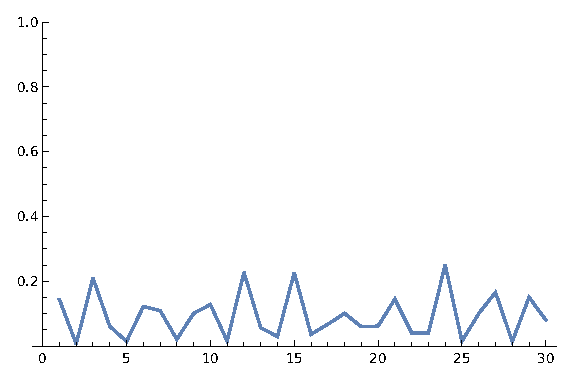
\includegraphics{PageRank_gr5.eps}

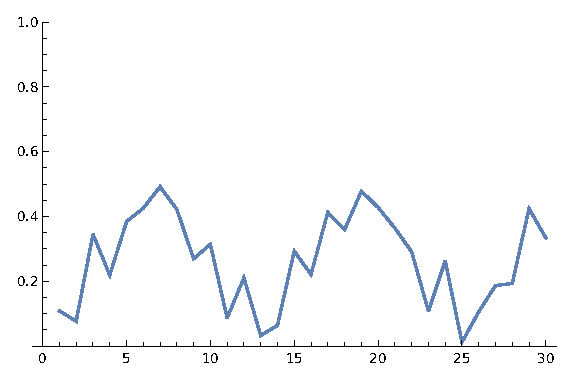
\includegraphics{PageRank_gr6.eps}

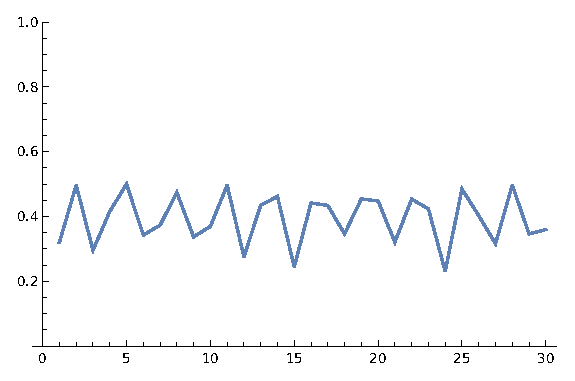
\includegraphics{PageRank_gr7.eps}

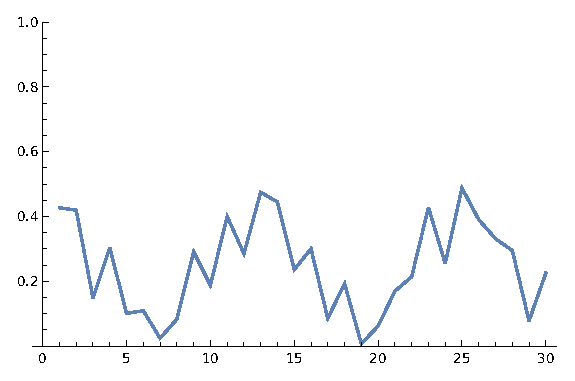
\includegraphics{PageRank_gr8.eps}

\end{document}
